\documentclass{article}
\usepackage[utf8]{inputenc}


\font\myfont=cmr12 at 25pt
%\title{\myfont Notes on Permanent Magnet Synchronous Machine (PMSM) Model %Predictive Control (MPC) and Operation Under Open Circuit Fault}
\font\hisfont=cmr12 at 15pt

\author{by \hisfont Hakan Saraç}
\date{}


\usepackage{float}
\usepackage{comment}
\usepackage{natbib}
\usepackage{graphicx}
\usepackage{indentfirst}
\usepackage{siunitx}
\usepackage{svg}
\usepackage{hyperref}
\usepackage{amsmath, bm}
\usepackage{graphicx} 
\usepackage{pstool}
\usepackage{listings}
\usepackage{natbib}
\usepackage{graphicx}
\usepackage{epstopdf}
\usepackage{tikz}
\usepackage[utf8]{inputenc}
\usepackage{pgfplots} 
\usepackage{pgfgantt}
\usepackage{pdflscape}
\pgfplotsset{compat=newest} 
\pgfplotsset{plot coordinates/math parser=false}
\lstloadlanguages{Matlab}%
\lstset{ 
	language=Matlab,                		% choose the language of the code
%	basicstyle=10pt,       				% the size of the fonts that are used for the code
	numbers=left,                  			% where to put the line-numbers
	numberstyle=\footnotesize,      		% the size of the fonts that are used for the line-numbers
	stepnumber=1,                   			% the step between two line-numbers. If it's 1 each line will be numbered
	numbersep=5pt,                  		% how far the line-numbers are from the code
%	backgroundcolor=\color{white},  	% choose the background color. You must add \usepackage{color}
	showspaces=false,               		% show spaces adding particular underscores
	showstringspaces=false,         		% underline spaces within strings
	showtabs=false,                 			% show tabs within strings adding particular underscores
%	frame=single,	                			% adds a frame around the code
%	tabsize=2,                				% sets default tabsize to 2 spaces
%	captionpos=b,                   			% sets the caption-position to bottom
	breaklines=true,                			% sets automatic line breaking
	breakatwhitespace=false,        		% sets if automatic breaks should only happen at whitespace
	escapeinside={\%*}{*)}          		% if you want to add a comment within your code
}

\addtolength{\oddsidemargin}{-.875in}
\addtolength{\evensidemargin}{-.875in}
\addtolength{\textwidth}{1.75in}
\addtolength{\topmargin}{-.875in}
\addtolength{\textheight}{1.75in}


\begin{document}
\title{\line(1,0){250}\\\myfont Embedded Environment Visualizer Library Handbook \\\line(1,0){250}}
\maketitle
\newpage
\tableofcontents
\newpage


\section{Introduction}


This document explains how to use the Embedded Environment Visualizer Library (EEVL). EEVL consists of three parts: two matlab routines and a library. These parts are called:
\begin{itemize}
	\item DataReceiver.m
	\item RawDataHandler.m
	\item MultipleFloatDataSender library
\end{itemize}

Each of these items are explained in the relevant section.
\newline

The aim of this library is to be able to collect, visualize and save data from an embedded environment, which is most of the time a trouble. 



\section{Matlab Routines} 
\subsection{DataReceiver.m} 

This routine is the main routine that collects, saves, plots the received data on the computer. 
\subsubsection{Options}
\label{subsubsection:Options}
This routine has several options, which are:
\begin{itemize}
	\item \textbf{EnableSaving :} This enables/disables the saving of the received data. The received data is tagged with date and hour information.
	\item \textbf{ProcessRawDataThresholdInBytes :} When this routine received \textbf{ProcessRawDataThresholdInBytes} bytes of data, the received data is processed plotted/saved.
	\item \textbf{EnablePlotting :} This enables/disables the plotting of the received data. The received data is being plotted with time axis. 
	\item \textbf{DataSampleRate (Hz):} This variable is used for determining the time axis of the plotting. It should match the data sending rate of the DSP.
	\item \textbf{TheSerialChannelDevice :} The serial channel port seen by the computer is stated in this variable. The port value can be determined from the device manager. For the example given in Figure \ref{fig:DeviceManager}, TheSerialChannelDevice should be set as 'COM5'.
\end{itemize}

\subsection{RawDataHandler.m}
The saved data by DataReceiver.m routine can be handled using this routine.
\subsection{Operation} TODO
After setting the options mentioned in \ref{subsubsection:Options}, this routine can be run in matlab.


\begin{figure}[H]
	\centering
	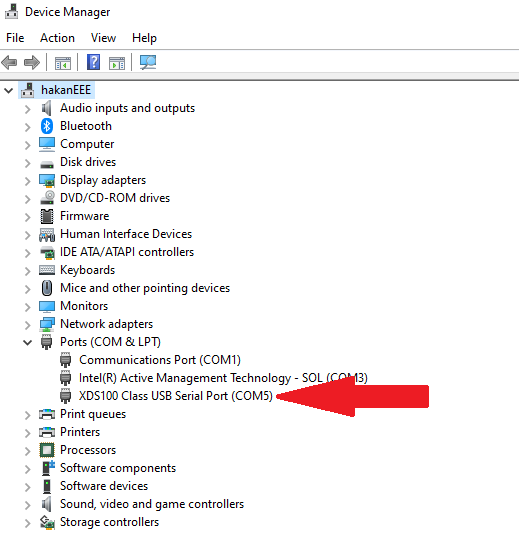
\includegraphics[scale=0.5]{Figures/DeviceManager.png}
	\caption{The serial port on the Device Manager screen}
	\label{fig:DeviceManager}
	\end{figure}

\subsection{Aim}

\section{MultipleFloatDataSender library}
This library is the critical part of the EEVL. For the embedded environment, all the necessary functions and/or variables are defined in this library. 


\bibliographystyle{plain}
\bibliography{references}
\end{document}
